\documentclass[11pt,a4paper]{article}
\usepackage[margin=20mm]{geometry}
\usepackage{graphicx,booktabs,xcolor,hyperref}
\definecolor{navy}{RGB}{24,65,98}
\hypersetup{colorlinks=true,urlcolor=navy,linkcolor=navy}
\setlength{\parindent}{0pt}\setlength{\parskip}{6pt}
\begin{document}
{\color{navy}\LARGE\bfseries PM12: four-channel CFD and TDC characterization}\par
{\large Incremental test chapter --- 10 November 2026}\par
\textbf{Board:} \texttt{PM12-K7-3A17A1B402212223}; EEPROM serial 1803.\\
\textbf{Populated channels:} 12, 10, 8 and 6.\\
\textbf{Run:} \texttt{pm12-cfd-four-20261110}.
\section*{Measured outcome}
The four TDC input paths passed finite-event and phase-response testing.
Every one of 25 input phases produced exactly 128 records on the selected
channel, with no events on the other eleven channels. All eight quiet windows
were empty. The scan contains 12,800 events, plus 64 mapping-discovery events.

\begin{center}\begin{tabular}{rrrr}\toprule
PM channel & RJ45 index & Slope [fine codes/ns] & Max. spread [fine codes RMS]\\\midrule
12 & 0 & -46.185 & 1.147 \\
10 & 1 & -46.201 & 1.185 \\
8 & 2 & -46.194 & 1.029 \\
6 & 3 & -46.177 & 1.083 \\
\bottomrule\end{tabular}\end{center}

Slope magnitudes differ by approximately 0.051\%. Timing is relative to the
programmed Kasli delay, assuming a 40.0787 MHz source. This is not an independent
calibration of absolute TDC timestamps or an intrinsic jitter measurement.

\section*{Fixture connections}
\begin{center}\begin{tabular}{rrrrr}\toprule
PM channel & DIOT slot & RJ45 index & CFD TX channel & Gate RX A/B\\\midrule
12 & 7 & 0 & 0 & 8/9\\
10 & 7 & 1 & 4 & 10/11\\
8 & 7 & 2 & 8 & 12/13\\
6 & 7 & 3 & 12 & 14/15\\\bottomrule
\end{tabular}\end{center}
Indices are zero based; Kasli occupies slot 0. HDMI remains on slot 6.
PM12 and Kasli use the shared LHC-derived reference. SFP0 is Kasli control LAN,
SFP1 the private PM link, and SFP2 the PM LAN bridge.

\section*{Acquisition procedure}
Check board identity and physical PGOOD; inhibit shared analog monitors.
Discover each CFD input with 16 pulses. Scan 25 serializer phases with 128
pulses each, one bit (approximately 1.0396 ns) per step, across 24.951 ns.
Freeze TDC buffers and download all channels through IPbus.
Separately, sweep each internal DAC-A through 101 codes from 0 to 65535,
recording all eight gate-return lanes with the Kasli ISERDES recorder.
The external MOD-DAC-28 and shared DMM were not used.

\newpage
{\color{navy}\Large\bfseries TDC input phase response}\par
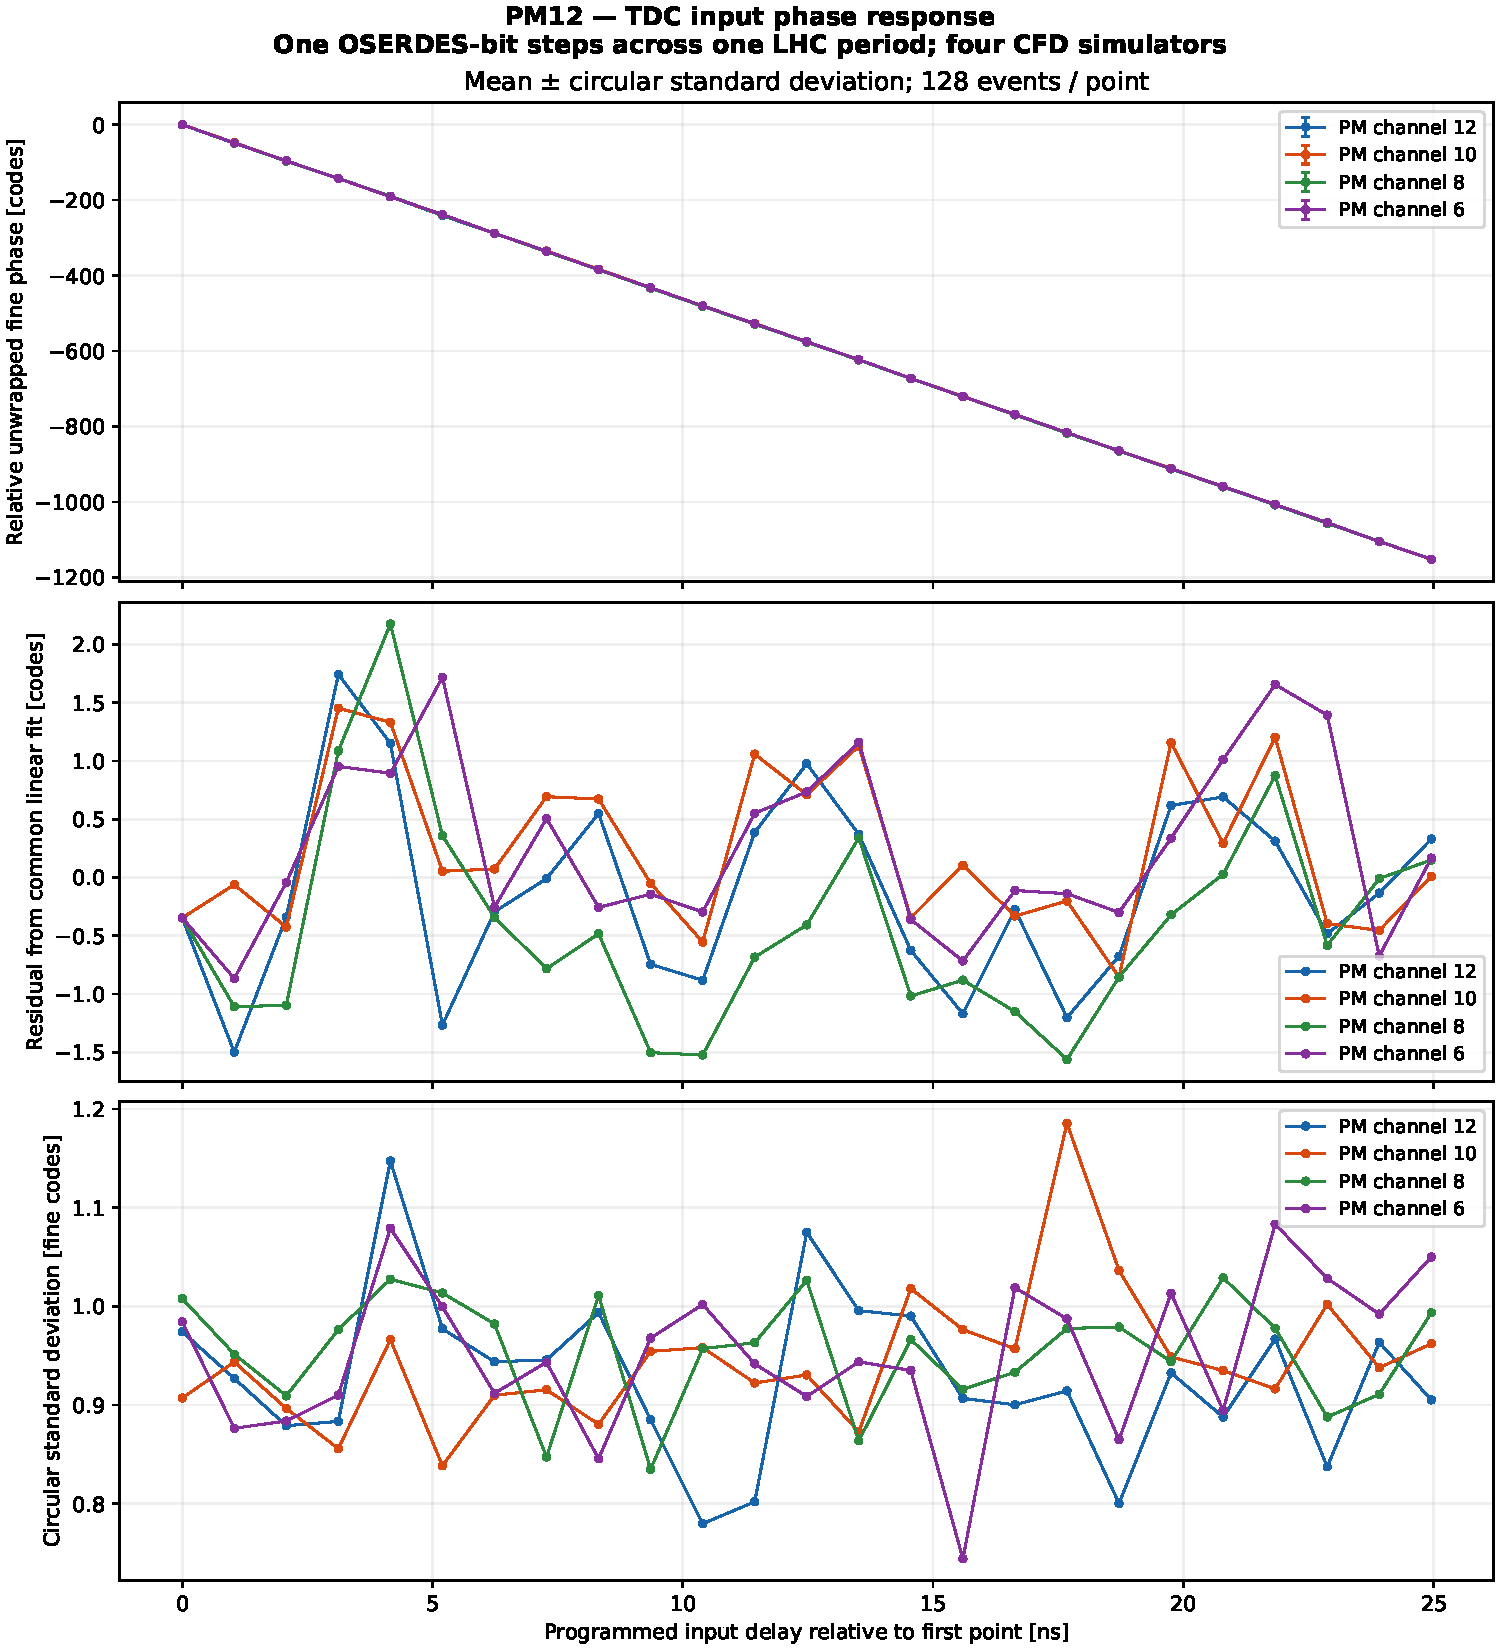
\includegraphics[width=\linewidth,height=.86\textheight,keepaspectratio]{tdc-phase-four.pdf}

Raw fine phase is unwrapped modulo 128 by nearest continuation. The middle
panel shows residuals from one common linear fit, exposing differences hidden
by the overlapping response curves. Coarse fields are retained separately.

\newpage
{\color{navy}\Large\bfseries Internal DAC-A phase-shifter response}\par
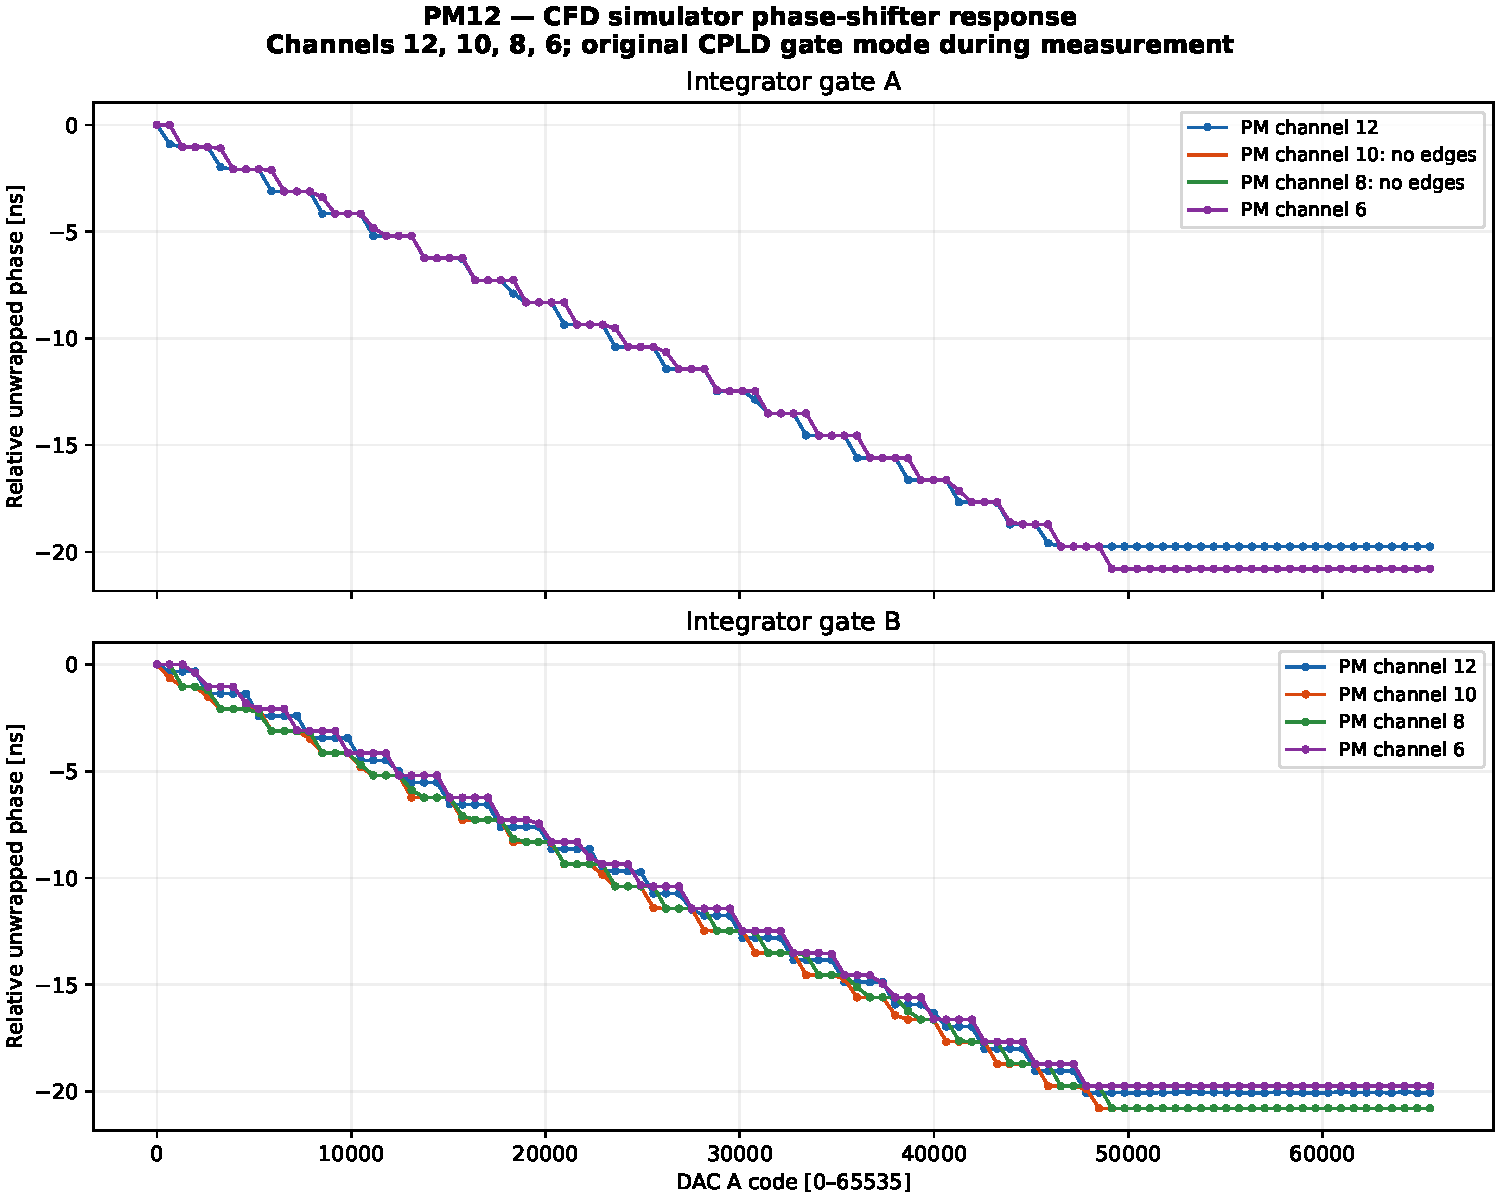
\includegraphics[width=\linewidth,height=.70\textheight,keepaspectratio]{gate-phase-four.pdf}

\textbf{Observed range:} approximately 20--21 ns, with a plateau near the upper
part of the DAC range (around code 48,000). The sampler bins are approximately
1.04 ns; fractional centroids do not establish calibrated sub-bin accuracy.

\textbf{Unresolved return-path findings:} INTA for PM channels 10 and 8 stayed
HIGH throughout the sweep. Their INTB returns respond to the corresponding DAC.
The observation does not locate the cause among driver, simulator, cabling,
repeater or receiver and is not a board-wide hardware PASS.

On channel 12, the prior INTB-off experiment suppressed the measured DAC-dependent
gate movement. Original complementary gates were temporarily restored for this
scan; the INTB-off CPLD12 image was restored and vendor-verified afterwards.

\newpage
{\color{navy}\Large\bfseries Evidence and retained hardware state}\par
\section*{Data integrity}
The 404 full-range DAC points contain 105,880,320 raw sampled bits.
During acquisition, 4,411,680 hardware phase records were checked against the
raw samples. All TDC raw counts and fine histograms were independently checked
against the downloaded binary files. The legacy single-port test also passed
with exactly 16 events on channel 12 after the four-port scan.

\section*{Build qualification}
The Kasli extension uses four independent output serializers and preserves
18 input serializers, HDMI and the three active SFP transceiver channels.
Dell Vivado 2025.2 qualification: setup slack 0.136 ns, hold slack 0.068 ns,
zero DRC errors. Physical CFD pin pairs were checked explicitly.

PM diagnostic bitstream SHA-256:\\
\texttt{1dbafd99033f803a086d4153ed3d873adfc9b4208b806785f00d3024bdfbf1ac}

Kasli four-port bitstream SHA-256:\\
\texttt{a71a08a258620b0e5a52c5d03aefd8c69040c9d15e8de6391c484ac182b7173b}

\section*{Final retained configuration}
PM image c7c42d28 and the new four-port Kasli image remain in FPGA SRAM.
CPLD12 retains INTB-off; the other eleven CPLD images are unchanged.
Internal DAC-A codes for channels 12/10/8/6 were explicitly restored to zero.
All shared monitor multiplexers are inhibited and both upstream I2C switches
are disconnected. CFD/HDMI outputs are off, port selection is zero, and both
DIO cards are inputs. TDC buffers are frozen and empty. ADC was not acquired
after restoration of the PM SRAM image. PGOOD and fresh FPGA DNA passed.

No MCU firmware, EEPROM, FPGA flash or PLL profile was written. The intended
CPLD12 gate-mode changes used vendor erase/program/verify procedures.
No external analog source or DMM was used. All hardware leases were released.

\section*{Editable sources and raw data}
This \texttt{report.tex} and both vector PDF/SVG figures are editable.
\texttt{gate-phase.csv}, \texttt{tdc-phase.csv} and \texttt{summary.json} contain
plot inputs and statistics. \texttt{raw-and-procedures.tar.gz} retains binary
buffers, raw phase captures, commands and exact executed procedures.
\texttt{gateware-artifacts.tar.gz} retains generated HDL, source snapshots,
qualified bitstreams, recovery images and qualification reports.
File hashes are listed in \texttt{sha256.json}.
\end{document}
